\cotefile{29}
\scanpage{115}
phisme évident
\margin{\figure{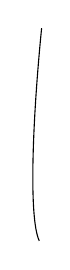
\begin{tikzpicture}\draw (.03,0) .. controls (-.08,-1.1) and (-.14,-2.4) .. (0,-2.7);\end{tikzpicture}}}
\[
\handwritten{\pi}_1^t(U_t)\handwritten{\rightarrow}\handwritten{\pi}_1^t(U)
\]
(un point-base géométrique de $U_t$ étant choisi). Cet homomorphisme est \uline{surjectif}.

Démonstration. Lorsqu'on remplace $L_t$ par $L_{t'}$ générique, alors la conclusion est contenue dans le corollaire 3, en d'autres termes, si $\unsure{\mathbb{U}|\deleted{V}U|\deleted{U}V|\mathbb{V}}$ est un revêtement étale \inserted{connexe} de $U$ \deleted{\unsure{tel que sa,}} (satisfaisant la condition de modération en\deleted{g}visagée - en fait, ce n'est pas nécessaire, enx vertu de 3 ) alors sa restriction $V_{t'}$ au dessus de $U_{t'}$ est connexe. On veut prouver que sa restriction $V_t$ au dessus de $U_t$ est \inserted{\handwritten{également}} connexe. Or pour un paramètre variable sur \inserted{\handwritten{un voisinage ouvert assez petit $T$ de}} la grassmanienne $\deleted{\unsure{T|G}}$ des $L_{t'}$\handwritten{,} \deleted{et voisin de $t$, la famill} \inserted{\handwritten{la}} famille des $Y_{t'}$ est un morphisme propre et lisse $Y\handwritten{\rightarrow}T$, et celle des $D_{t'}$ est un sous-schéma fermé \deleted{de} $\handwritten{\Delta}$ de $Y$, qui est la réunion d'un sous-schéma $\handwritten{\Delta}_1$ qui est de codi\unsure{\deleted{mem}men|\deleted{men}mem}sion $\handwritten{\geq}2$ sur chaque fibre (et qui ne comp\unsure{\deleted{t}|t}e\inserted{\handwritten{\unsure{m|nt|n}}} pas, à cause du théorème de pureté relative) et d'un diviseur $\handwritten{\Delta_2}$ à croise\`{m}ents normaux relatifs. Le revêtement donné $V$ de $U$ définit un revêtement \deleted{$V$ de $Y$} $V'$ de $U'=Y-\handwritten{\Delta}$, et il\deleted{f} faut montrer que la restriction de celui-ci à la fibre géométrique de $t$ est connexe, sachant qu'il en est ainsi de sa restriction à la fibre géométrique en $t'$, la générisation maximale de $t$. Or par la pureté, on sait que $V'$ se prolonge en un revêtement étale $V''$ de $U''=Y-\handwritten{\Delta_2}$, et par hypothèse ce dernier est modérément ramifié sur les fibres, relativement au diviseur $\handwritten{\Delta_2}$. La conclusion est alors une conséquence du théorème \deleted{\unsure{connu}} de spécialisation pour le groupe fondamental modéré, qui figure(ra) dans SGA 1 XIII (exposé de Mme Raynaud).

\uline{Remarque}7.Avec les notations de SGA 7 XVIII\handwritten{,} 6 s'applique pour tout pinceau de Lefschetz $D$ pour fournir la surjectivité de\deleted{s quotients par}
% archive sheet number: 114

\scanpage{116}
l'homomorphisme $\handwritten{\pi}_1^t(D-\overset{\handwritten{\scriptscriptstyle\vee}}{D})\handwritten{\rightarrow}\handwritten{\pi}_1^t(\unsure{\mathbb{P}|\deleted{R}P}-\overset{\handwritten{\scriptscriptstyle\vee}}{X})$, et donne le théorème de conjugaison des cycles évanescents (donc le théorème d'irréductibilité de la cohomologie évanescente) pourvu qu'on ne soit pas dans le cas $\operatorname{car}.k=2$ et $\dim X$ impaire (NB \deleted{ce n'est pas,} dans la situation du th. de Griffiths, il n'y a donc pas d'ennui). Dans ce dernier cas, par contre, je ne sais \deleted{rien} pas prouver\inserted{la conjuga\unsure{\deleted{n}i|i}son sous $\handwritten{\pi}_1(D-\overset{\handwritten{\scriptscriptstyle\vee}}{D})$}, sauf pour un pinceau \uline{générique}, puisqu'alors la représentation envisagée est sauvage; \inserted{j'ignore si \unsure{ella|elle|\deleted{cela}\handwritten{elle}} reste vrai\handwritten{\unsure{e}} pour un pinceau \uline{général}.} Noter cependant que la conjugaison des sous-groupes de monodromie locale\deleted{\unsure{,|s}} \uline{dans} $\operatorname{Aut}(H^{n-1}\handwritten{(Y_{\bar{\eta}}))}$ (qui est très élémentaire) reste vraie, bien entendu, et celle-ci suffit pour prouver le théorème que j'ai proposé (au par. 6 de XVIII) caractérisant le cas où la condition (A) n'est \uline{pas} vérifiée.
% archive sheet number: 115

\scanpage{119}
% archive sheet number: 119

\handwritten{2}. Supposons donné une situation $(Y,V,H,V')$ analogue à $(X,\handwritten{U},G,U')$, et un morphisme $f:X\handwritten{\longrightarrow}Y$ tel que $f(U)\handwritten{\longrightarrow}f(V)$, un morphisme $f':U'\handwritten{\longrightarrow}V'$ compatible avec $U\handwritten{\longrightarrow}V$ induit par $f$, un morphisme de groupes $\handwritten{\phi}:G\handwritten{\longrightarrow}H$ tel que \deleted{$\unsure{f'(gx')=}$} $f'$ soit compatible avec les actions de $G$ et $H$ via $\handwritten{\phi}$, \deleted{et}

Le cas le plus courant sera celui où on se donne un point géométrique $a$ de $U$, \inserted{d'où} un point géométrique $b$ \inserted{$=f(a)$} de $V$, où $U'$ et $V'$ sont respectivement des quotients des revêtements universels de $U$ et $V$ basés en $a$ et $b$, $G$ et $H$ étant respectivement des quotients de $\handwritten{\pi}_{1}(U,a)$ et $\handwritten{\pi}_{1}(V,b)$, l'homomorphisme $f':U'\handwritten{\longrightarrow}V'$ étant induit par les homomorphismes canoniques sur les revêtements universels en $a$ resp. $b$\deleted{\unsure{;|,} \unsure{un tel} $\unsure{f'}$} \unsure{\inserted{\deleted{ainsi que $\handwritten{\phi}$}}} \deleted{\unsure{est} \unsure{donc} déterminé de}, \deleted{façon unique $G$ et $H$ étant les g} $\handwritten{\phi}:G\handwritten{\longrightarrow}H$ étant induit par $f_{\handwritten{*}}:\handwritten{\pi}_{1}(U,a)\handwritten{\longrightarrow}\handwritten{\pi}_{1}(\unsure{\deleted{B}V|\deleted{V}B},b)$ ; de cette façon $f'$ et $\handwritten{\phi}$ sont déterminés sans ambiguïté par $f$, et leur existence signifie simplement que $f_{\handwritten{*}}:\handwritten{\pi}_{1}(U,a)\handwritten{\longrightarrow}\handwritten{\pi}_{1}(V,b)$ veut bien passer au quotient en un $\handwritten{\phi}:G\handwritten{\longrightarrow}H$ (i.e. applique un certain sous-groupe dans un certain sous-groupe). Considérons d'autre part le localisé strict $\handwritten{\overline}{Y}$ de $Y$ en le point géométrique $f(\handwritten{\bar}{x})$ de $Y$, d'où \deleted{\unsure{un}} $\handwritten{\bar}{V},\handwritten{\bar}{V}'$ comme dessus; supposons donné un prolongement $\handwritten{\overline}{Y'}$ de $\handwritten{\bar}{V}'$ en un schéma à groupe d'opérateurs $H$ sur $\handwritten{\bar}{Y}$, et supposons donné enfin un homomorphisme $\handwritten{\overline}{f'}:\handwritten{\overline}{X'}\handwritten{\longrightarrow}\handwritten{\overline}{Y'}$ qui prolonge l'homomorphisme \deleted{\unsure{ft|f'}} $\handwritten{\overline}{U'}\handwritten{\longrightarrow}\handwritten{\overline}{V'}$ induit par $f'$. Pour tout point $\handwritten{\xi}$ de $\handwritten{\overline}{X'}_{\handwritten{\bar}{x}}$, $\handwritten{\overline}{f'}(\handwritten{\xi})$ est alors un point\deleted{s} de $\handwritten{\overline}{Y'}_{\handwritten{\bar}{y}}$, et on peut considérer le groupe d'inertie correspondant $H_{\handwritten{\overline}{f'}(\handwritten{\xi})}$. On a alors la relation évidente
\[
\handwritten{\phi}(G_{\handwritten{\xi}})\handwritten{\subset}H_{\handwritten{\overline}{f'}(\handwritten{\xi})}\ .
\tag*{\handwritten{(2.1)}}
\]
Dans le cas où le\deleted{s} groupe $G$ resp. $H$ opère transitivement sur $\handwritten{\overline}{X'}_{\handwritten{\bar}{x}}$ resp. $\handwritten{\overline}{Y'}_{\handwritten{\overline}{y'}}$, on peut donc dire que $\handwritten{\phi}$ \inserted{applique tout groupe \deleted{de}} \deleted{transforme la classe de conjugaison de sous-groupes} d'inertie de $G$ rel. à $x$ \inserted{\handwritten{\uline{dans}} un groupe d\deleted{e}\handwritten{'}} \deleted{\unsure{en|à} la classe de conj. des sous-groupes} d'inertie de $H$ rel à $y=f(x)$.

\deleted{D'autre part} Il reste alors à expliciter l'homomorphisme $\handwritten{\overline}{f'}:\handwritten{\overline{X'}\longrightarrow\overline{Y'}}$.

\figure{\handwritten{\begin{tikzpicture}[x=0.006cm,y=-0.006cm]
\draw[gray,line width=0.3pt] (1664,451) .. controls (1622,413) and (1571,429) .. (1514,436) .. controls (1119,456) and (709,433) .. (276,428);
\draw[gray,line width=0.3pt] (258,438) .. controls (270,417) and (240,422) .. (228,451) .. controls (206,521) and (206,664) .. (202,870) .. controls (201,912) and (214,941) .. (218,979) .. controls (230,1065) and (230,1149) .. (211,1200) .. controls (236,1219) and (296,1206) .. (347,1208) .. controls (591,1211) and (732,1211) .. (901,1210) .. controls (950,1208) and (976,1188) .. (969,1152) .. controls (1209,1140) and (1415,1155) .. (1601,1137);
\draw[gray,line width=0.3pt,->] (211,1200) .. controls (186,1269) and (152,1426) .. (156,1546) .. controls (153,1742) and (178,1921) .. (203,1996) .. controls (212,2022) and (250,2009) .. (309,2019);
\draw[gray,line width=0.3pt] (63,532) -- (42,549) .. controls (33,559) and (36,583) .. (47,596);
\end{tikzpicture}}}

\scanpage{120}
% archive sheet number: 119

En pratique, il sera vrai que $\handwritten{\overline}{U'}$ est schématiquement dense dans $\handwritten{\overline}{X'}$\inserted{et $\handwritten{\overline}{Y'}$ séparé sur $\handwritten{\bar}{Y}$}, de sorte que $\handwritten{\overline}{f'}$ sera déterminé de façon unique en termes des autres données, comme l'unique prolongement de $\handwritten{\overline}{U'}\handwritten{\longrightarrow}\handwritten{\overline}{V'}$ induit par $f'$; ce sera le cas en particulier dans le cas envisagé plus haut où $\handwritten{\overline}{X'}$ se déduit de \deleted{$\handwritten{\bar}{\unsure{U}}$} $\handwritten{\overline}{U'}$ par normalisation. Bien entendu\deleted{\unsure{r}}, pour pouvoir conclure\inserted{\handwritten{alors}} que tout sous-groupe d'inertie de $G$ rel. à $x$ s'envoie dans un sous-groupe d'inertie de $H$ rel. à $y$, il faudra avoir vérifié l'\uline{existence} d'un p\deleted{p}rolongement $\handwritten{\overline}{f'}$ de $\handwritten{\overline}{U'}\handwritten{\longrightarrow}\handwritten{\overline}{V'}$\inserted{\handwritten{(la commutation aux actions de $G$ dev. alors \uline{automatique})}}. \handwritten{cela \unsure{marchera}, en interprétant $\unsure{\overline{f'}|f'}$ comme $\overline{X'}\unsure{\longrightarrow|-}\overline{Y'}\mathbin{\times}_{\bar Y}\overline{X'}$, lorsque $\overline{Y'}$ est \uline{entier} \deleted{\illegible{1}} sur $\bar Y$, cf. EGA II 6.1.14.}

\handwritten{3.} Revenons à la situation de 1), supposons que $\underline{O}_{X,x}$ soit un anneau local régulier, et que $\handwritten{\bar}{U}$ soit le complémentaire dans le schéma stricte\deleted{\unsure{men}}ment local régulier $\handwritten{\bar}{X}$ d'un diviseur \inserted{$\handwritten{\bar}{D}$} à croisements normaux. On est en particulier dans le cas favorable où la définition de $\handwritten{\overline}{X'}$ est immédiate par normalisation. Supposons que la ramification de $\handwritten{\overline}{U'}$ en les points maximaux de $\handwritten{\bar}{D}$ soit \uline{modérée}. On sait alors, par le calcul local bien connu, que pour tout $\handwritten{\unsure{\xi|\zeta}\in}\handwritten{\overline}{X'}_{\handwritten{\bar}{x}}$, le groupe d'inertie correspondant $G$ s'identifie canoniquement \deleted{au groupe} à un groupe quotient du groupe
\margin{\handwritten{$C=$ l'ensemble des composantes irred. de $\bar D$}}
\[
I=\handwritten{\prod}_{\handwritten{\unsure{\ell|l}\ne}p}\underline{Z}_{\handwritten{\ell}}(1)(k(\handwritten{\bar}{x}))^C=\handwritten{\prod}_{\handwritten{\ell\ne}p}T_{\handwritten{\ell}}(k(\handwritten{\bar}{x}\unsure{)}\ )^C\ ,
\tag*{(3.1)}
\]
$p$ étant la caractéristique résiduelle en $x$. De p\deleted{\unsure{m}}lus, ce même calc\uline{u}l local montre que le facteur de ce groupe d'inertie correspondant à la composante $\handwritten{\bar}{D}_c$ $(c\handwritten{\in}C)$ du diviseur de ramification $\handwritten{\bar}{D}$ coïncide aussi avec le groupe d'inertie relatif à n'importe quel point de $\handwritten{\overline}{X'}$ au dessus du point maximal de $\handwritten{\bar}{D}_c$ (ou de tout autre point de $\handwritten{\bar}{D}_c$ qui n'appartient à aucune autre composante irréductible de $\handwritten{\bar}{D}$) qui générise $\handwritten{\xi}$ ; comme il y a toujours de tels points, cela montre que la classe de conjugaison du facteur en question peut aussi s'interpréter comme la \deleted{grou} classe des groupes d'inertie en les points envisagés de $\handwritten{\bar}{D}_c$ ; en particulier, cette classe de conjugaison ne dépend que de la composante irréductible de $D=X-U$ \deleted{, image} de point générique l'image du point générique de $\handwritten{\bar}{D}_{\handwritten{c}}$.

\scanpage{121}

\handwritten{4.} Revenons à la situation de 2, et supposons que la structure de $(\handwritten{\bar}{X},\handwritten{\bar}{U})$ soit celle envisagée dans 3, et que de même $\handwritten{\bar}{Y}$ soit un schéma local régulier et $\handwritten{\bar}{V}=\handwritten{\bar}{Y}-\operatorname{supp}\handwritten{\bar}{E}$, $\handwritten{\bar}{E}$ étant un diviseur à croisements normaux sur $\handwritten{\bar}{Y}$. Soit $C'$ l'ensemble des composantes irréductibles de $\handwritten{\bar}{E}$, On voit alors que pour tout $c'\handwritten{\in}C'$, l'image inverse de $\handwritten{\bar}{E}_{c'}$ est un diviseur sur $\handwritten{\bar}{X}$ dont le support est contenu dans celui de $\deleted{\unsure{E}}\handwritten{\bar}{D}$, donc est de la forme
\[
\handwritten{\bar}{f}(\handwritten{\bar}{E}_{c'})=\handwritten{\sum}_{c}\unsure{a|n}_{c,c'}\handwritten{\bar}{D}_c\ ,
\]
où pour $c'$ fixé, les $n_{c,c'}$ sont des entiers $\handwritten{\geq}0$ non tous nuls. Ces notations fixées, un calcul immédiat \deleted{\unsure{direct}} d'images inverses de revêtements kummériens montre que pour deux points correspondants $\handwritten{\xi}$ et $\handwritten{\eta}$, \deleted{l'homom} on a commutativité dans le diagramme
\diagram{\(\handwritten{(4.1)}\qquad\)
\begin{tikzcd}[ampersand replacement=\&,column sep=large,row sep=large]
\&\handwritten{\deleted{\unsure{H_\xi|G_\xi}}}\&G_{\handwritten{\xi}}^{\handwritten{\deleted{\unsure{\xi|x}}}}\handwritten{\arrow}[r,"{\handwritten{\phi}}","{\deleted{\unsure{N|\phi}}}"']\&H_{\handwritten{\eta}}\\
\handwritten{-}\&{}\handwritten{\arrow}[u,gray]\&\handwritten{\prod}_{\handwritten{\unsure{\ell|l}}}\underline{Z}_{\handwritten{\ell}}(1)(\handwritten{\bar}{x})^C\handwritten{\arrow}[u]\handwritten{\arrow}[r,"N"]\&\handwritten{\prod}^{\handwritten{\prime\prime}}_{\handwritten{\ell}}\underline{Z}_{\handwritten{\ell}}(1)(\handwritten{\bar}{y})^{C'}\handwritten{\arrow}[u]
\end{tikzcd}\(\ ,\)}
les flèches \deleted{horizontales}\inserted{verticales} étant les épimorphismes canoniques, et $N$ étant l'homomorphisme défini par la matrice $N=(n_{c,c'}\handwritten{)}_{(c,c')\handwritten{\in}C\mathbin{\times}C'}$, compte tenu que l'homomorphisme $k(\handwritten{\bar}{y})\handwritten{\longrightarrow}k(\handwritten{\bar}{x})$ induit des isomorphismes
\[
\underline{Z}_{\handwritten{\ell}}(1)(\handwritten{\bar}{y})\handwritten{\xrightarrow{\sim}}\underline{Z}_{\handwritten{\ell}}(1)(\handwritten{\bar}{x})\ .
\]
Pour que \inserted{l'homomorphisme} $N$ soit un isomorphisme, il est donc nécessaire et suffisant que \inserted{$\operatorname{card}C=\operatorname{card}C'$ et que} \deleted{det $N$} l'entier ordinaire $\text{dét }N$ soit égal à $\pm p^r$, où $p$ est l'exposant caractéristique de $k(x)$ et $k(y)$; dans ce cas, on conclut donc que les \inserted{sous-}groupes d'inertie de $H$ en $y$ sont les conjugués des images des \inserted{sous-}groupes d'inertie de $G$ en $x$.

\margin{\handwritten{$\bar E=\unsure{Y^{\vee}|\check Y}$}}
5. Supposons en particulier que l'on ait $V=Y-\operatorname{supp}E$, $E$ étant un diviseur \inserted{$\handwritten{\geq}0$} sur $Y$, \deleted{tel que} $U=f^{\handwritten{-1}}(V)$, et que \deleted{pour tout $\unsure{x\handwritten{\in}}f^{\handwritten{-1}}(E)$, posant} les conditions suivantes soient satisfaites:

\inserted{\handwritten{a) Pour $x\in f^{-1}(\operatorname{supp}E)$, $y=f(x)$, $\underline{O}_{X,x}$ et $\underline{O}_{Y,y}$ sont noethériens.}}

\deleted{\unsure{a}}\handwritten{b}) Le diviseur \inserted{\handwritten{$D=$}} $f^{\handwritten{*}}(E)$ est défini, c'est un sous-schéma \uline{régulier} de
% archive sheet number: 120
